
\subsection{研究背景}

\subsubsection{Mesa3D显示列表绘制模式实现原理}

显示列表绘制模式即glGenList/glNewList/glEndList/glCallList,它可以提高性能,因为它存储OPENGL的函数,供以后使用,如果需要多次重绘同一个几何图形,或者如果一次需要多次调用的用于更改状态的函数,把这些函数存储在显示列表中,此时将显示列表中的矩阵结果集保存,后续使用不需要重复计算以提高性能。显示列表更像是命令缓存器,而不是动态数据库,也就是说当显示列表创建后,就无法修改。同时显示列表的创建也存在一定的系统开销,因此一个小的显示列表未必会提升性能。

我们以下面所示的svPerfGL测试集里面的显示列表模式为例,来看一下Mesa3D图形库是如何实现显示列表的绘制模式的。

\begin{lstlisting}
 // Create Display List
 glNewList(trianglesListIndx, GL_COMPILE);
 glDrawArrays(GL_TRIANGLES, 0, tNumVerts);
 glEndList(); 

 // Call Display List
 glCallList(trianglesListIndx);
\end{lstlisting}


当执行glNewList时,Mesa3D图形库会执行alloc\underline{ }vertex\underline{ }store函数预分配大小为VBO\underline{ }SAVE\underline{ }BUFFER\underline{ }SIZE*sizeof(GLfloat)的空白VRAM空间,这个空间我们姑且称之为buffer0。在显示列表机制下,保存模式的glDrawArrays只会执行一次,目的是将所有的顶点属性(位置、法线和颜色等)写入buffer0。VBO\underline{ }SAVE\underline{ }BUFFER\underline{ }SIZE的初值是8*1024,只能存放8*1024/3=2730个顶点属性,而glDrawArrays可能需要写入更多的顶点属性,因此buffer0是远远不够存放这些顶点属性的。当buffer0溢出后,显示列表会继续分配大小为VBO\underline{ }SAVE\underline{ }BUFFER\underline{ }SIZE * sizeof(GLfloat)的buffer1,buffer2,buffer3...直到所有顶点属性都写入VRAM。可见,当glDrawArray执行完时,所有的顶点属性已经存入VRAM,但是分散在很多个小buffer中。

接着通过执行glCallList来调用已保存好顶点属性的显示列表,glCallList将执行vbo\underline{ }save\underline{ }playback\underline{ }vertex\underline{ }list函数来实现渲染,该函数调用r600\underline{ }draw\underline{ }vbo向GPU发如下命令:

\begin{lstlisting}
cs->buf[cs->cdw++] = PKT3(PKT3_DRAW_INDEX_AUTO, 1, 
                          rctx->predicate_drawing);
cs->buf[cs->cdw++] = info.count;
cs->buf[cs->cdw++] = V_0287F0_DI_SRC_SEL_AUTO_INDEX 
                     | (info.count_from_stream_output? 
                        S_0287F0_USE_OPAQUE(1) : 0);
\end{lstlisting}

这些命令通过Command Stream机制被GPU读取并执行,从而启动pipeline进行3D渲染。

\begin{figure}[H] 
  \centering
  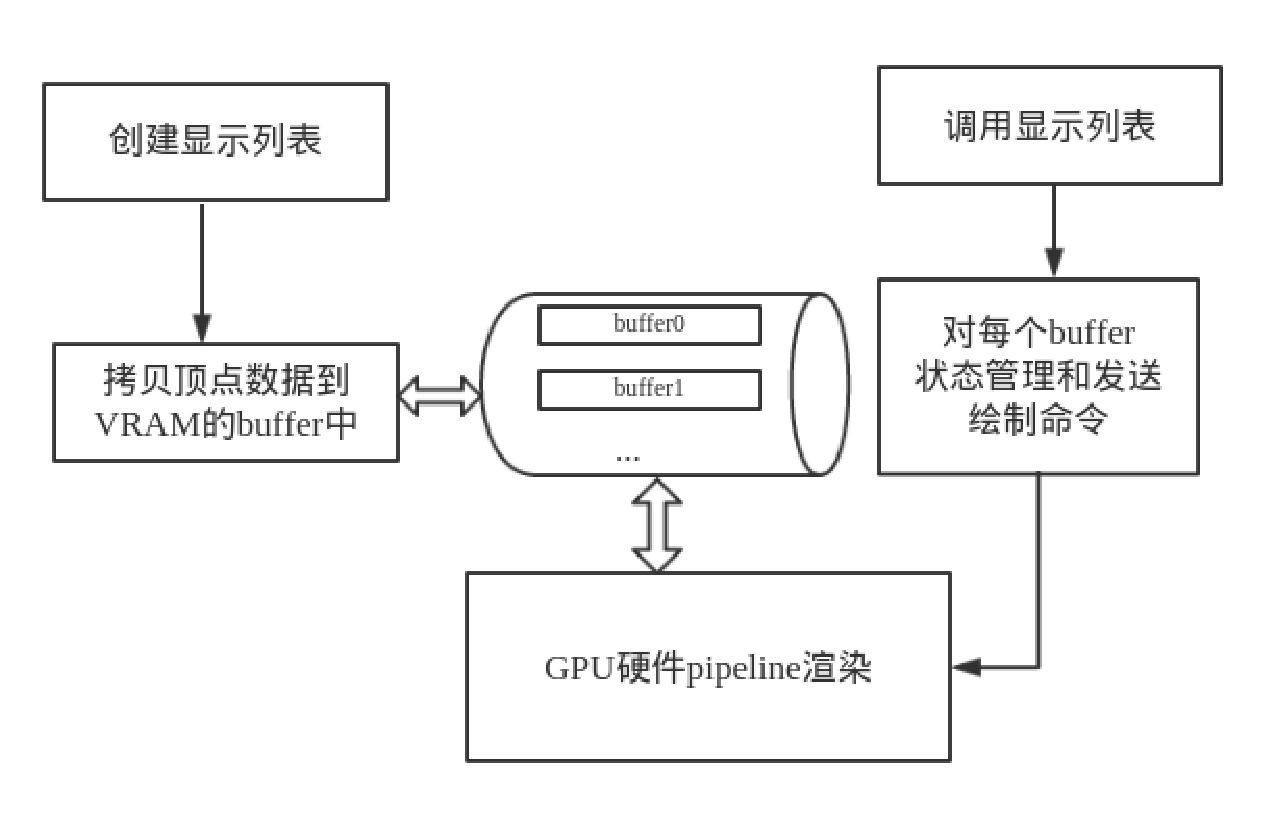
\includegraphics[width=12cm,height=10cm]{figures/chap03/display-list-flow}
  \caption{Mesa3D图形库显示列表实现机制}
  \label{fig:display-list-flow}
\end{figure}

由于显示列表是一次创建多次调用,所以如图\ref{fig:display-list-flow}所示,每次在调用显示列表时候都会做对每个buffer进行状态管理和发送绘制命令到GPU。GPU在执行完3D渲染之后将结果放入framebuffer中然后通过显示设备显示出来。

\subsubsection{Mesa3D立即模式绘制模式实现原理}

为了说明Mesa3D立即模式的实现原理,这里以svPerfGL的立即模式测试项为例展开分析:

\begin{lstlisting}
	glBegin(GL_TRIANGLES);
	for (i=0; i<tNumVerts; i++){
		glNormal3fv((GLfloat *)(tNorms+i));
		glColor3fv((GLfloat *)(tColors+i));
	    glVertex3fv((GLfloat *)(tVerts+i));
	}
	glEnd();
\end{lstlisting}

这里在一对glBegin和glEnd中间放入了大量的绘制命令,Mesa3D在调用glBegin时候首先会根据绘制图形样式,配置好info.mode信息,例如V\underline{ }008958\underline{ }DI\underline{ }PT\underline{ }POINTLIST、V\underline{ }008958\underline{ }DI\underline{ }PT\underline{ }TRILIST等等。接着会在VRAM上创建一个大小为VBO\underline{ }VERT\underline{ }BUFFER\underline{ }SIZE的空白VRAM空间,这里同样称为buffer0。VBO\underline{ }VERT\underline{ }BUFFER\underline{ }SIZE的默认值为1024*64。接着glBegin与glEnd中间的相关顶点数据就会通过宏函数ATTR(A, N, T, V0, V1, V2, V3)拷贝到buffer0中,当buffer0装满数据后,Mesa3D会备份边界顶点数据,然后将绘制命令发送给GPU进行渲染:

\begin{lstlisting}
r600_write_config_reg(cs, R_008958_VGT_PRIMITIVE_TYPE,
                      r600_conv_pipe_prim(info.mode));
cs->buf[cs->cdw++] = PKT3(PKT3_DRAW_INDEX_AUTO, 1, 
                          rctx->b.predicate_drawing);
cs->buf[cs->cdw++] = info.count;
cs->buf[cs->cdw++] = V_0287F0_DI_SRC_SEL_AUTO_INDEX |
                     (info.count_from_stream_output? 
                         S_0287F0_USE_OPAQUE(1) : 0);
\end{lstlisting}

之后创建新的buffer1来处理后续的顶点数据,如此反复直到glBegin和glEnd里面的数据全都装载完毕并交给GPU处理。简单来说整个过程就是如图\ref{fig:immediate-mode-flow}所示。这里与图\ref{fig:display-list-flow}里面的显示列表实现机制的不同在于显示列表机制下只需要进行一次的数据装载,以后每次调用显示列表时候就不必再数据装载了,而立即模式下每次调用都需要重新的数据装载。

\begin{figure}[H] 
  \centering
  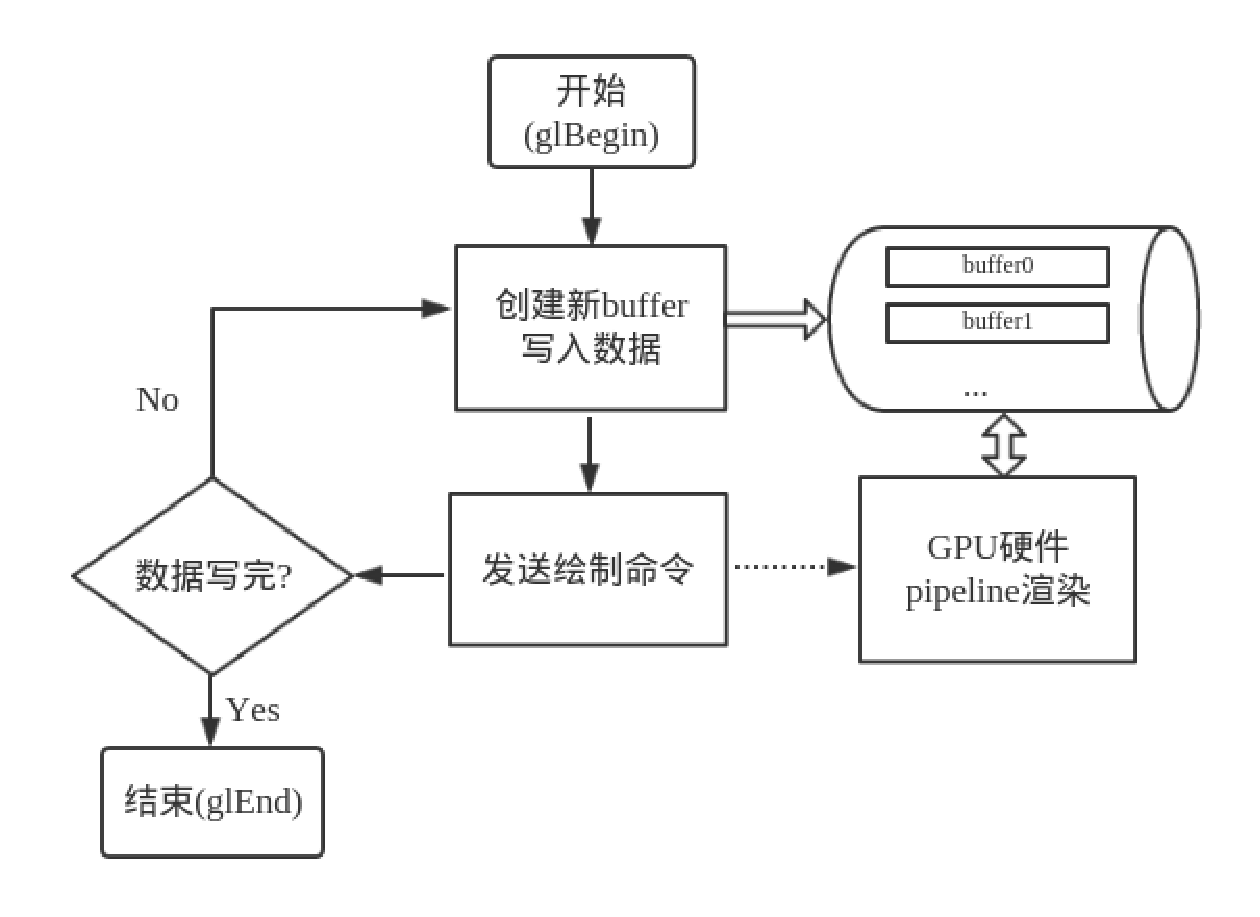
\includegraphics[width=14cm,height=10cm]{figures/chap03/immediate-mode-flow}
  \caption{Mesa3D图形库立即模式实现机制}
  \label{fig:immediate-mode-flow}
\end{figure}

\subsubsection{Mesa3D顶点数组绘制模式实现原理}
从前面的立即模式实现原理我们可以看到顶点数据是一个个的搬运到VRAM上的buffer上的,当我们绘制拥有大量数据的图形时候,这样一点点的搬运就显得非常的缓慢了,当然我们可以尝试使用显示列表来对这些数据进行预编译,需要遍历这些顶点数据然后把数据传给GPU的显存。但是这些数据不一定是静态的,有可能在我们每次渲染的时候,我们需要对这些数据进行更改。这个时候就不适合使用显示列表了。

为了很好的解决这个问题。我们可以使用顶点数组,我们可以随时进行预编译或修改几何图形,然后一次性传输这些数据。顶点数组的绘制模式相对于立即模式极大的提高了绘制效率。使用顶点数组有3个基本的步骤:

\begin{itemize}
\item{} 激活(启用)最多可达8个数组,每个数组用于存储不同类型的数据: 顶点坐标,表面法线,颜色等等。
\item{} 把数据放入数组中。这些数组是通过它们的内存位置的地址(即指针)进行访问。
\item{} 用这些数据绘制几何图形。OpenGL通过指针从所有激活的数组中获取数据。
\end{itemize}

我们还是以svPerfGL的顶点数组模式测试项为研究对象来分析Mesa3D顶点数组的实现原理:

\begin{lstlisting}
glEnableClientState(GL_VERTEX_ARRAY);
glVertexPointer(3, GL_FLOAT, sizeof(float)*3, (const GLvoid *)tVerts);
glEnableClientState(GL_NORMAL_ARRAY);
glNormalPointer(GL_FLOAT, sizeof(float)*3, (const GLvoid *)tNorms);
glEnableClientState(GL_COLOR_ARRAY);
glColorPointer(3, GL_FLOAT, sizeof(float)*3, (const GLvoid *)tColors);

glDrawArrays(GL_TRIANGLES, 0, tNumVerts);
\end{lstlisting}

这里在介绍Mesa3D顶点数组实现原理之前先介绍一个重要的数据结构:
\begin{lstlisting}
struct pipe_vertex_buffer{
   ...
   struct pipe_resource *buffer; 
   const void *user_buffer;
};

struct pipe_vertex_buffer vertex_buffer[PIPE_MAX_ATTRIBS];
\end{lstlisting}
这里vertex\underline{ }buffer数组就是存放着各个属性数据数组的指针,当我们使用传统的立即模式时候,这些指针就指向着前面一节说到的VRAM上的buffer(struct pipe\underline{ }resource *buffer),而在我们使用顶点数组模式时候,这些指针就指向着我们用户准备的顶点数据数组(const void *user\underline{ }buffer)。所以在顶点数组模式下,在glVertexPointer()这类函数执行时候,Mesa3D会把用户指定的数组指针添加到对应vertex\underline{ }buffer[]数组里面的user\underline{ }buffer中。接着我们调用glDrawArrays()之类的函数进行顶点数组模式绘制时候,Mesa3D会执行u\underline{ }vbuf\underline{ }upload\underline{ }buffers函数将用户定义的顶点数组数据通过memcpy()函数从内存拷贝到显存中,然后像之前的立即模式一样向GPU发送绘制命令执行硬件渲染。

\begin{figure}[H] 
  \centering
  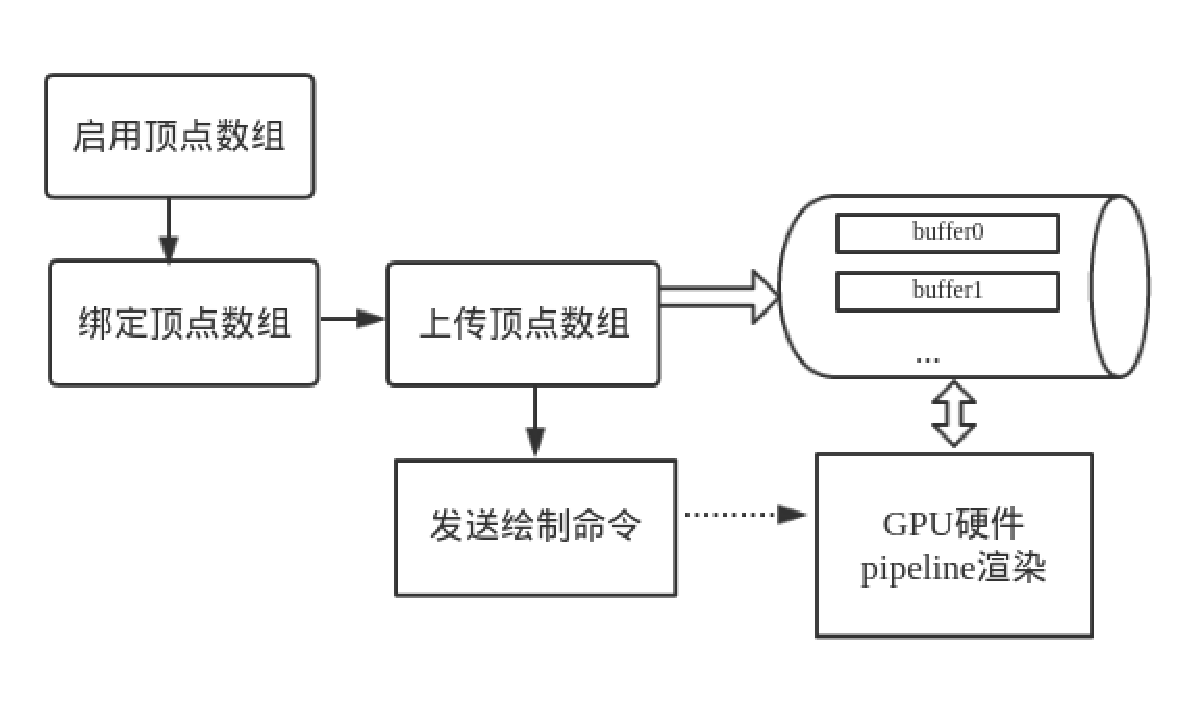
\includegraphics[width=12cm,height=8cm]{figures/chap03/vbo-flow}
  \caption{Mesa3D图形库顶点数组模式实现机制}
  \label{fig:vbo-flow}
\end{figure}

顶点数组模式绘制的简要流程如图\ref{fig:vbo-flow}所示,这里需要说明的是顶点数组模式下在VRAM上创建的buffer大小是依据用户定义的数组大小而定的,并不像立即模式那样有着固定的大小,一旦填满就开始部分绘制,顶点数组模式是把所有数据都传递到显存之后再一次性的GPU绘制,由于是一次性memecpy的大数据传输,所以传输效率上要比传统的立即模式快的多,这也是后来OpenGL标准中增加顶点数组模式的原因。

\subsection{Mesa3D图形库CPU与GPU负载分析}

\subsection{Mesa3D图形库CPU与GPU负载平衡优化}
